\documentclass[12pt,oneside,a4paper]{article}
 
\def\projecttype{Лабораторная работа }% тип работы
\def\projectno{2}% номер работы, если есть
\def\projectname{Основы вакумной техники}% название
\def\perenos{10}% Если название 1 строка то 14, если 2 то 12 и тд может менятся от шрифта 
\def\name{\href{https://t.me/mali_na}{Малиницкий Дмитрий}}% автор

 
\usepackage{listings}

\lstset{
    language=C++,
    basicstyle=\small\ttfamily,
    keywordstyle=\color{blue},
    commentstyle=\color{green},
    stringstyle=\color{red},
    numbers=left,
    numberstyle=\tiny,
    breaklines=true,
    breakatwhitespace=true,
    tabsize=4,
    frame=single,
    captionpos=b,
    showstringspaces=false,
}
 \usepackage[%
  a4paper,%
  left = 20mm,%
  right = 20mm,%
  textwidth = 178mm,%
  top = 40mm,%
  bottom = 30mm,%
  %heightrounded,%
  headheight=70pt,%
  headsep=25pt,%
]{geometry}
\usepackage{graphicx}
\usepackage[sfdefault,light]{FiraSans}
\usepackage{hyperref}
\hypersetup{ colorlinks = true, allcolors  = link-blue, }
\usepackage{lastpage}
\usepackage{graphicx}
\usepackage{float}
\usepackage{xspace}
\usepackage{longtable}
\usepackage{tabularx}
\usepackage{color,colortbl}
\usepackage[english,russian]{babel}
\usepackage{lipsum}
\usepackage{amsmath}
\usepackage{xcolor}
\usepackage{amssymb}



\definecolor{link-blue}{RGB}{6,69,173}
\definecolor{dark-green}{RGB}{52,133,62}
\definecolor{light-blue}{RGB}{127,180,240}
\definecolor{dark-blue}{RGB}{72,120,224}
\definecolor{heading-grey}{RGB}{128,128,128}
\definecolor{heading2-grey}{RGB}{200,200,200}
\definecolor{Critical}{RGB}{192,0,0}
\definecolor{High}{RGB}{255,0,0}
\definecolor{Medium}{RGB}{255,192,0}
\definecolor{Low}{RGB}{255,255,0}
\definecolor{Informational}{RGB}{94,185,255}






\usepackage{listings}
\usepackage{enumitem}
\usepackage{array,booktabs}
\usepackage{fancyhdr}
\renewcommand{\footrulewidth}{0.2pt}
\renewcommand{\headrulewidth}{0.2pt}
\fancyfoot{}
\fancyhead{}
\fancyfoot[C]{Confidential}
\fancypagestyle{plain}{
    \fancyfoot[C]{\\ \textcolor{heading-grey}{\newline Page \thepage\ of \pageref{LastPage}}}
    \fancyhead[R]{\includegraphics[width=5cm]{imgmain/hselogo_international_line.png}}
}
\fancypagestyle{fancy}{
    \fancyfoot[C]{\\ \textcolor{heading-grey}{\newline Page \thepage\ of \pageref{LastPage}}}
    \fancyhead{}
}
\thispagestyle{fancy}\pagestyle{plain}

\newcommand{\email}[1]{\href{mailto://#1}{#1}}
\newcommand{\newchapter}[1]{{\section*{#1}
\addcontentsline{toc}{chapter}{#1}}}
\newcommand{\newsection}[1]{{\subsection*{#1}
\addcontentsline{toc}{section}{#1}}}
\newcommand{\newsubsection}[1]{{\subsubsection*{#1}
\addcontentsline{toc}{subsection}{#1}}}
\usepackage[skip=10pt plus1pt, indent=0pt]{parskip}

\usepackage{etoolbox}
\makeatletter
\patchcmd{\chapter}{\if@openright\cleardoublepage\else\clearpage\fi}{}{}{}
\makeatother
\makeatletter
\renewcommand\tableofcontents{%
    \if@twocolumn
      \@restonecoltrue\onecolumn
    \else
      \@restonecolfalse
    \fi
    \section*{\contentsname
        \@mkboth{%
           \MakeUppercase\contentsname}{\MakeUppercase\contentsname}}%
    \@starttoc{toc}%
    \if@restonecol\twocolumn\fi
    }
\makeatother

\usepackage{titlesec}

\titleformat{\section}
{\normalfont\huge\bfseries}{\thesection}{1em}{}
\titleformat{\subsection}
{\normalfont\Large\bfseries}{\thesubsection}{1em}{}
\titleformat{\subsubsection}
{\normalfont\large\bfseries}{\thesubsubsection}{1em}{}

% \titleformat{command}[shape]{format}{label}{sep}{before}[after]
% \titlespacing{command}{left spacing}{before spacing}{after spacing}[right]

\titlespacing{\section}{0pt}{1em}{0.5em}
\titlespacing{\subsection}{0pt}{0em}{0.25em}

\usepackage[T1]{fontenc}
\renewcommand*\oldstylenums[1]{{\firaoldstyle #1}}
\usepackage[europeanresistors,americaninductors]{circuitikz}

\begin{document}

\renewcommand{\headrulewidth}{0pt}

\renewcommand{\thesection}{\arabic{section}}

%%%%%%%%%%%%%%%%%%%%%%%%%%%%%%%%%%%%%%%%%
%%          Begin title page           %%
%%%%%%%%%%%%%%%%%%%%%%%%%%%%%%%%%%%%%%%%%

\begin{titlepage}
  \thispagestyle{empty}
   \thispagestyle{fancy}
   \begin{center}
        \vspace*{8em}
   
        \centering\includegraphics[width=13cm]{imgmain/hselogo_international_line.png}

        \vspace{3em}

        \Huge{\textsc{\projecttype  \projectno \\ \projectname}}

        \vspace{\perenos em}
        
   \Large {\today \\ \name}
      
   \end{center}


\end{titlepage}

\renewcommand{\headrulewidth}{0.2pt}

\newpage



%%%%%%%%%%%%%%%%%%%%%%%%%%%%%%%%%%%%%%%%%
%%           Begin contents            %%
%%%%%%%%%%%%%%%%%%%%%%%%%%%%%%%%%%%%%%%%%
\parindent=0.5cm




\tableofcontents

\newpage

\section{Оборудование}

Для выполнения лабораторной работы потребуется следующее оборудование:
\begin{enumerate}
    \item Вакуумные камеры с фланцами ISO-K-100.
    \item Заглушки ISO-K-100 для вакуумных камер.
    \item Вентили с фланцами ISO-KF-16.
    \item Манометрические преобразователи ПМТ-2 и ПМИ-2 с переходниками ISO-KF-25.
    \item Цифровые датчики вакуума Thyracont.
    \item Цифровой вакуумметр Мерадат-ВИТ.
    \item Соединительные провода.
    \item Источник постоянного напряжения на 24 В.
    \item Турбомолекулярный откачной пост.
    \item Спиральный безмасляный насос.
\end{enumerate}


\section{Теоретическая часть}

\subsection{Основы вакуумной техники}
Многие направления современных физических исследований требуют использования вакуумной техники. Вакуумные условия необходимы для напыления пленок и металлических контактов высокого качества, приготовления чистой поверхности для исследования свойств материалов, работы ускорителей элементарных частиц, обеспечения вакуумной теплоизоляции.

\subsection{Основное уравнение вакуумной техники}
Ключевые параметры вакуумной техники могут быть оценены на основе элементарной кинетической теории газов. Основные формулы:

\textbf{Средняя длина свободного пробега (\( \lambda \)):}
\begin{equation}
    \lambda = \frac{1}{\pi \sqrt{2}n(2r)^2}
\end{equation}

\textbf{Среднее время образования моноатомного слоя (\( \tau \)):}
\begin{equation}
    \tau = \frac{4a}{nv}
\end{equation}


\textbf{Средняя скорость молекул газа (\( v \)):}
\begin{equation}
    v = \sqrt{\frac{8k_BT}{\pi m_0}}
\end{equation}

\textbf{Давление газа (Закон идеального газа):}
\begin{equation}
    p = nk_BT % Вставьте здесь формулу
\end{equation}

\textbf{Диапазоны давления:}
\begin{itemize}
    \item Низкий вакуум: $1000 - 1$ мбар
    \item Средний вакуум: $1 - 10^{-3}$ мбар
    \item Высокий вакуум: $10^{-3} - 10^{-7}$ мбар
    \item Ультравысокий вакуум: $10^{-7} - 10^{-14}$ мбар
\end{itemize}

\subsection{Компоненты вакуумной системы}
Типовая вакуумная система состоит из откачиваемого объема, линий откачки, вакуумного насоса, вентилей напуска и датчиков вакуума.

\textbf{Откачиваемый объем:}
\begin{itemize}
    \item Характеризуется давлением, объемом, количеством и потоком газа.
\end{itemize}

\textbf{Линии откачки:}
\begin{itemize}
    \item Пропускная способность линии (\( C \)):
    \begin{equation}
        C = \frac{Q_{pv}}{\Delta p}; \quad \frac{1}{C}=\frac{1}{C_1}+\frac{1}{C_2}+\ldots 
    \end{equation}
\end{itemize}

\subsection{Типы вакуумных насосов}

Вакуумные насосы классифицируются по различным принципам работы, каждый из которых подходит для конкретных условий и требований. Ниже приведены основные типы:

\begin{enumerate}
    \item Адсорбционные и криогенные насосы - используют адсорбцию газа на поверхности твёрдого вещества или конденсацию газа при очень низких температурах для достижения вакуума. Работают при любых давлениях, достигая сверхвысокого вакуума.
    \item Магнитные электроразрядные насосы - в этих насосах для перемещения газа используются магнитные поля, они не имеют движущихся частей и обеспечивают сверхвысокий вакуум.
    \item Ионно-сорбционные насосы - сочетают в себе ионизацию газа с его последующей адсорбцией на поверхности, что позволяет достигать высокого вакуума.
    \item Турбомолекулярные насосы - работают на принципе передачи количества движения от быстро вращающихся лопаток к молекулам газа, удаляя их из насоса.
    \item Паромасляные и диффузионные электронные насосы - используют пары масла или жидкого металла для создания вакуума посредством диффузии газов через пар.
    \item Двухроторные (Рутса) насосы - представляют собой вращающиеся насосы с двумя роторами, которые сжимают и переносят газ без масла.
    \item Ротационные пластинчатые насосы - в этих насосах используются вращающиеся пластины для перекачивания газа, они могут использоваться как для достижения предварительного, так и для среднего вакуума.
    \item Спиральные насосы - это вариант ротационного насоса, где используются спирально нарезанные роторы для перекачивания газа.
\end{enumerate}


\subsubsection{Турбомолекулярный насос}
Турбомолекулярный насос основан на принципе механического удаления молекул газа с помощью высокоскоростной турбины. Эти насосы развивают скорость вращения турбины до примерно 1000 оборотов в секунду, что позволяет эффективно передавать молекулам газа импульс в направлении откачки. Важной особенностью такого насоса является необходимость начального создания форвакуумных условий, для чего используется форвакуумный насос. Это предотвращает повреждение механических компонентов насоса, особенно лопаток турбины и осевых подшипников, которые могут быть повреждены при запуске при атмосферном давлении. При внезапном росте давления в уже откачанном объеме, соединенном с насосом, также возможно повреждение элементов турбины, что делает использование форвакуумного насоса критически важным для безопасной эксплуатации турбомолекулярного насоса.

\subsubsection{Спиральный насос}
Спиральный безмасляный форвакуумный насос имеет уникальную конструкцию, состоящую из неподвижной и вращающейся спиральных платформ. При вращении платформы газ, находящийся в рабочем объеме насоса, сжимается и вытесняется, что приводит к снижению давления. Эти насосы способны работать без использования масла, что предотвращает загрязнение вакуумной системы. Спиральные насосы идеально подходят для создания предвакуума и часто используются в комбинации с турбомолекулярными насосами, чтобы обеспечить оптимальные условия для их работы. Принцип действия спирального насоса обеспечивает надежное и эффективное снижение давления, что делает его важным элементом в системах создания вакуума.


\subsection{Датчики вакуума}

Вакуумные системы часто оснащаются различными типами датчиков для точного измерения давления. Ниже представлены основные типы датчиков вакуума:

\begin{enumerate}
    \item \textbf{Гидростатические датчики} - они используют жидкостный манометр для определения давления, основываясь на высоте столба жидкости, которая изменяется в зависимости от давления газа.
    \item \textbf{Деформационные датчики} - преобразуют механическую деформацию, вызванную давлением газа, в электрический сигнал для измерения уровня вакуума.
    \item \textbf{Компрессионные датчики} - измеряют давление посредством изменения объема газа, что позволяет точно определить вакуум.
    \item \textbf{Тепловые датчики} - используют термопары или терморезисторы для измерения изменений в теплопроводности газа, которые коррелируют с его давлением.
    \item \textbf{Ионизационные датчики} - определяют вакуум через количество ионов, создаваемых электронным пучком в ионизированном газе.
    \item \textbf{Электроразрядные датчики} - наблюдают за электрическим разрядом в газе, который изменяется в зависимости от давления, позволяя таким образом измерять вакуум.
    \item \textbf{Инверсно-магнитные датчики} - эти датчики используют изменение магнитных свойств газа под действием вакуума для измерения очень низких давлений.
\end{enumerate}


\section{Практическая часть}
\subsection{Предельное давление}
Соберем установку, подключим датчики, поставим камеры для съёмки. Снимем зависимость показания датчиков от времени. Потом откроем их и обработаем данные.
\newpage
\begin{figure}
    \centering
    \includegraphics[width=1\linewidth]{Снимок экрана 2023-11-20 в 01.45.48 (2).png}
    \caption{Обработка данных}
    \label{fig:enter-label}
\end{figure}

Во время обработки данных воспользуемся динамическим шагом, первые точки с быстрым изменением мы будем промерять каждую секунду, последующие с частотой в плоть до 1 измерения в 2 минуты. Итого получим $264$ значения зависимости давления на обоих датчиков от времени. Данные находятся тут. 

Далее напишем код на \href{https://github.com/FriendBobik/MKT2}{Python}, который построит график зависимости давления от времени для каждого датчика, так как в начальный момент они очень сильно различаются, построим так же отдельно первые 50 точек, вторые 50 точек, ну и отдельно оставшиеся точки. Получим вот такую "систему графиков"
\newpage
\begin{figure}[!ht]
    \centering
    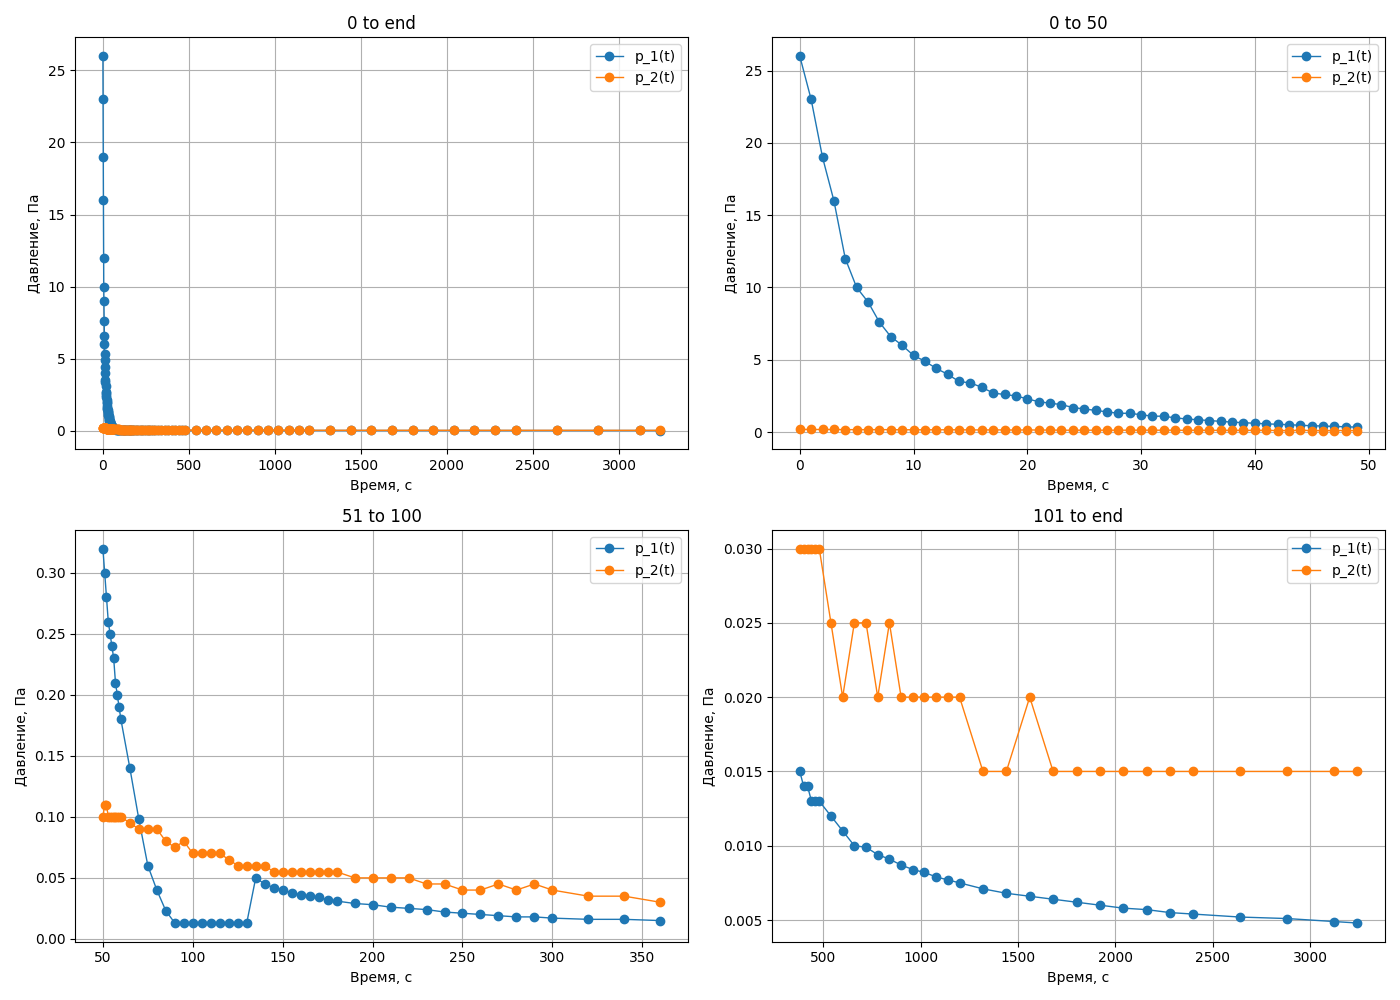
\includegraphics[width=1\linewidth]{garf_1.png}
    \caption{Показания датчиков}
    \label{fig:enter-label2}
\end{figure}

Здесь оранжевая линия, это датчик \href{https://thyracont-vacuum.com/en/artikelnummer/dn-16-iso-kf-vsp63dl-en/}{VSP63DL (пьезорезистивный)}, а синяя линия, это комплекс из 2 датчиков ПМТ-2 (термопарный) и ПМИ-2 (ионизационный). Стоит упомянуть, что от 85 до 135 секунды происходило переключение датчиков, то есть до 85 секунды показания теплового, а после ионизационного. Так как датчик VSP63DL, предназначен для широкого диапазона давлений,  а тепловой и ионизационный датчик, для более узких диапазонов. Из этого мы можем сделать вывод, что показания синей линии более верное, и исходя из этого мы можем оценить минимальное давление как:

$$4.3 \pm 0.05 \cdot 10^{-3} \textbf{ Па}$$

\subsection{Определение скорости откачки}

Для определения динамики процесса откачки вакуума используется логарифмическая зависимость скорости откачки от времени. Скорость откачки \( S \) определяется как отношение объема откачиваемого воздуха \( V \) к времени откачки \( t \), умноженное на логарифм отношения начального \( p_1 \) и конечного \( p_2 \) давлений в системе:

\begin{equation}
S = \frac{V}{t} \ln\left(\frac{p_1}{p_2}\right)
\end{equation}

Экспериментально полученный объем вакуумной камеры составляет около 2000 см\(^3\), однако из-за ограничений методики невозможно точно определить абсолютный объем, что вносит погрешность в измерения. Имея данные о начальном и конечном давлении, можно построить графики, которые визуализирую эффективность откачки от времени. Мы будем использовать только показания датчиков ПМТ-2 и ПМИ-2, ввиду их большей точности.


\begin{figure}[!ht]
    \centering
    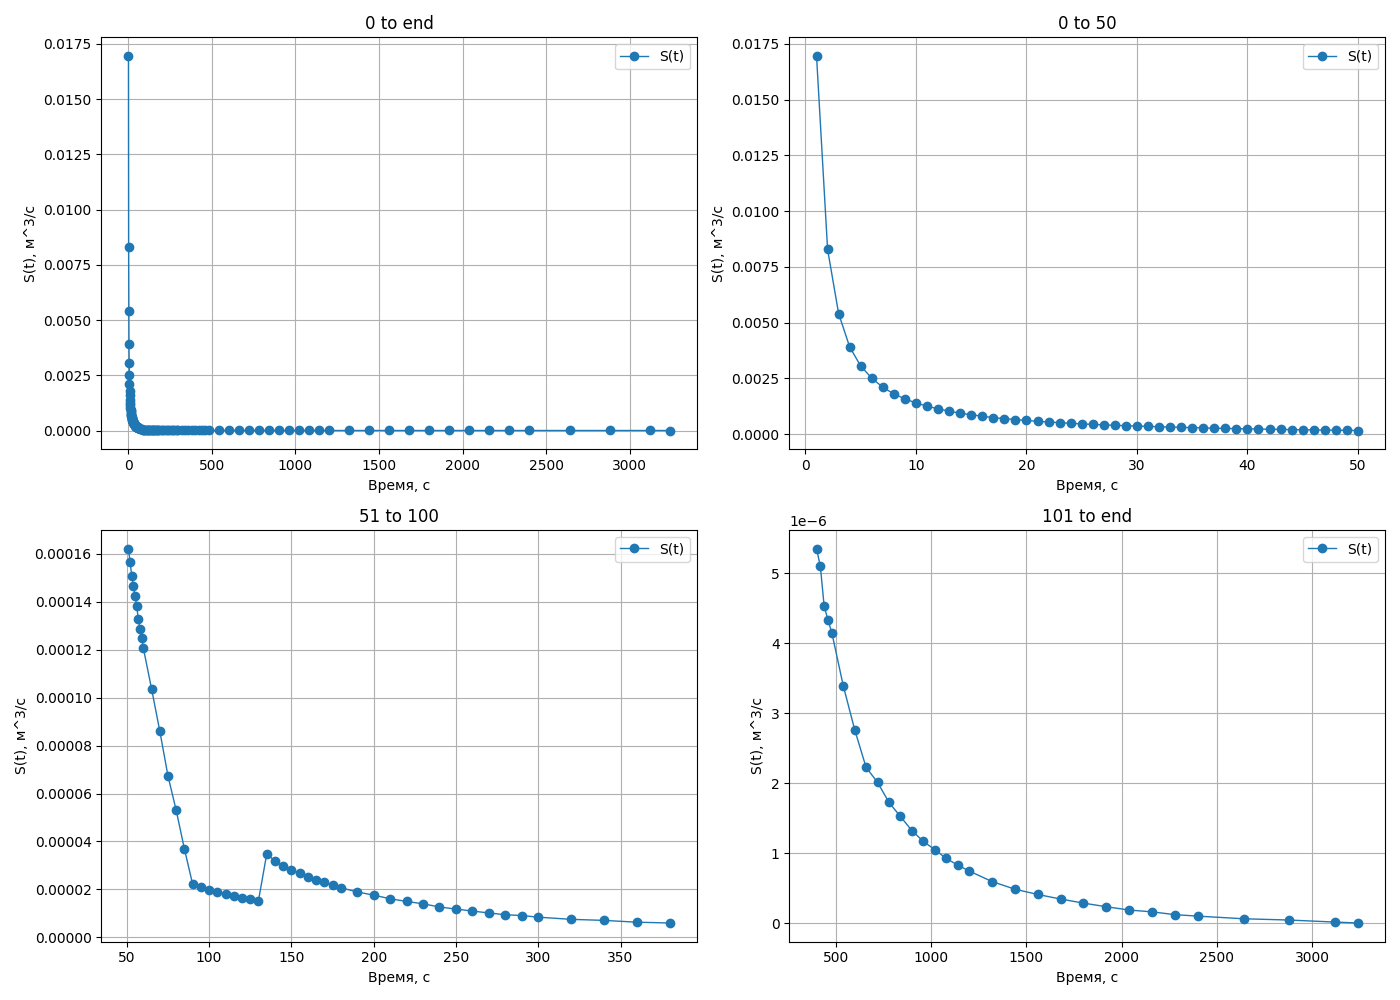
\includegraphics[width=1\linewidth]{garf_2.png}
    \caption{Зависимость скорости откачки от давления}
    \label{fig:enter-label3}
\end{figure}
\subsection{Скорость натекания}

Выполним всё то же самое как для скорости натекания газа в систему.

Получим график:
\newpage
\begin{figure}[!ht]
    \centering
    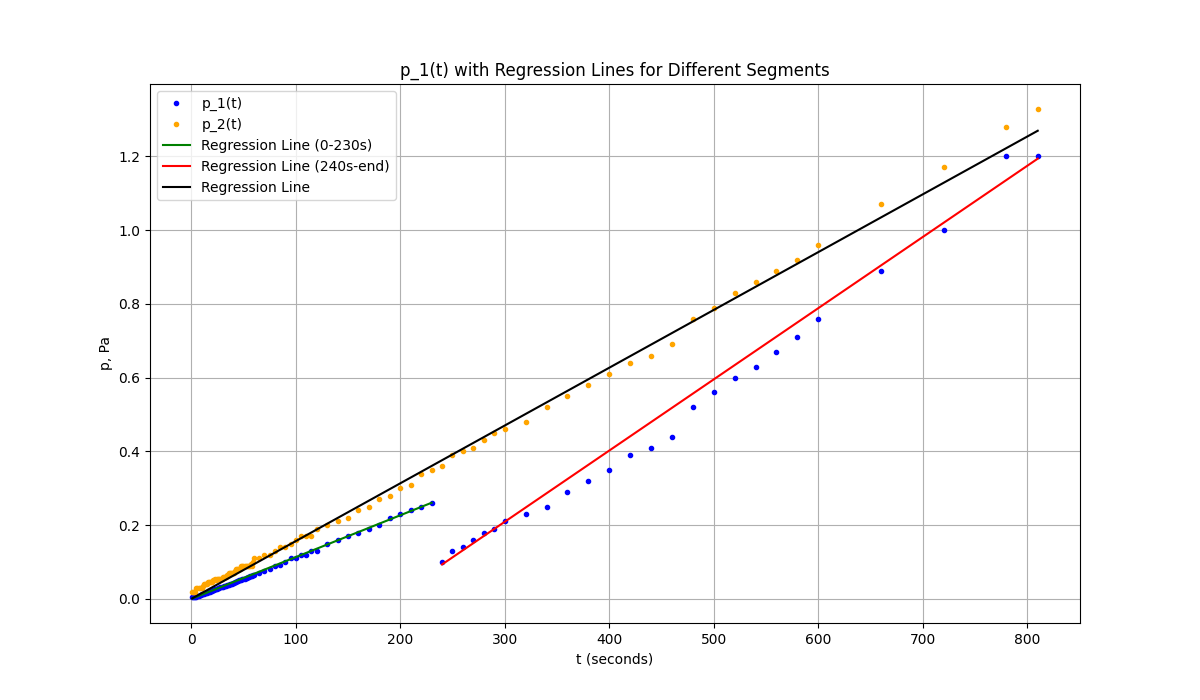
\includegraphics[width=1\linewidth]{garf_3.png}
    \caption{График скорости натекания}
    \label{fig:enter-label}
\end{figure}

 Где синее точки показания датчиков ПМТ-2 и ПМИ-2, а оранжевые VSP63DL, так же проведена аппроксимация, по красной линии, скорость утекания:

 $$0.00193 \quad m^3/c$$
 
По зеленой

$$0.00113  \quad m^3/c$$

По черной:

$$0.00156 \quad m^3/c$$






\end{document}
       